
\documentclass[handout,12pt,dvipsnames,t]{beamer}
\setbeamertemplate{footline}[frame number]
\title{Statistical Practice in Epidemiology 2018}
\subtitle{Survival analysis with competing risks} % \\[10mm]
\author{Janne Pitk\"aniemi (EL) }
\date{}
\usepackage{Sweave}
\begin{document}
\Sconcordance{concordance:Survival_competing_risk.tex:Survival_competing_risk.Rnw:%
1 7 1 1 0 804 1}


\maketitle


\begin{frame}[fragile]
\frametitle{Points to be covered}

\begin{itemize}
\item[1.] Survival or time to event data \& censoring.
 \medskip
 \item[2.] 
 Competing risks: event-specific cumulative incidences \& hazards.
 \medskip
\item[3.] Kaplan--Meier and Aalen--Johansen estimators.
 \medskip
 \item[4.] 
 Regression modelling of hazards: Cox model.
 \medskip
 \item[5.]
 Packages \texttt{survival, mstate, cmprisk}.
\medskip
\item[6.] 
 Functions \texttt{Surv(), survfit(), plot.survfit(), coxph(), Cuminc()}.
\end{itemize}

\end{frame}


\begin{frame}[fragile]
\frametitle{Survival time -- time to event}

\textbf{Time} spent (\texttt{lex.dur}) in a given \textbf{state} (\texttt{lex.Cst}) from its 
beginning till a certain \textit{endpoint} or \textit{outcome} \textbf{event}  (\texttt{lex.Xst}) or \textit{transition}  occurs, changing the state to another. \\
 

\bigskip
Examples of such times and outcome events:
\begin{itemize}
\item lifetime: birth $\rightarrow$ death,
\medskip
\item duration of marriage: wedding $\to$ divorce, 
\medskip
\item healthy exposure time: \\ start of exposure  
  $\rightarrow$ onset of disease,
  \medskip
\item clinical survival time: \\
 diagnosis of a disease  $\rightarrow$ death.
\end{itemize}


\end{frame}


\begin{frame}[fragile]
\frametitle{Ex. Survival of 338 oral cancer patients}

% Dataset \texttt{oralca.txt} describes the 
% Survival of patients with oral squamous cell
% carcinoma, treated at a tertiary level hospital. 
{Important variables}: 
\begin{itemize}
\item \texttt{time} = duration of patientship from \\ 
 diagnosis (\textbf{entry}) till death (\texttt{death}) or censoring (\texttt{Alive}),
 (\texttt{lex.Cst} is (\texttt{Alive}))
\medskip
\item
\texttt{event} = indicator for the outcome and its \\
 observation at the end of follow-up (\textbf{exit}): \\
  0 = censoring,  \\
  1 = death from oral cancer\\
%  1 = death from oral cancer, \\
%  2 = death from some other cause.
\end{itemize}
% \texttt{Surv(time, event)} creates a \emph{survival} object.

\medskip
Special features:
\begin{itemize}
\item
   Two possible endpoints
   \medskip
\item
   Censoring -- incomplete observation of the survival time.   
\end{itemize}
\end{frame}

\begin{frame}
   \frametitle{Set-up of classical survival analysis} 

\begin{itemize}
\item
\textbf{Two-state model}: only one type of event changes the initial state.
\medskip
\item
Major applications: analysis of lifetimes
 since birth and of survival times since diagnosis of a disease 
 until death from any cause.
\end{itemize}

\setlength{\unitlength}{0.7pt}
% \begin{center}
\begin{picture}(400,80)(-40,70)
  \thicklines
  \put(  0, 80){\framebox(110,50){Alive}}
  \put(240, 80){\framebox(110,50){Dead}}
  \put(240, 80){\makebox(110,40)[b]{\scriptsize{(lex.Xst = 1 or 2)}}}
  \put(125,105){\vector(1, 0){100}}
  \put(170,110){\makebox(0,0)[b]{Transition}}
\end{picture}
% \end{center}

\begin{itemize}
\item
 \textbf{Censoring}: Death and final lifetime not observed
  for some subjects 
  %, as the follow-up terminates 
  due to emigration or closing the follow-up while they are still
 alive 
\end{itemize}

\end{frame}
  

\begin{frame}[fragile]

\frametitle{Distribution concepts: hazard function}

The \textbf{hazard rate} or \textbf{intensity} function $\lambda(t)$
\begin{align*}
\lambda(t) & = 
 {P(t < T \le t+\Delta | T > t)}/{\Delta}, \ for small \Delta 
\end{align*}
\begin{itemize}
\item[$\approx$]  the conditional probability that
the event occurs in a short
 interval $(t, t+\Delta]$, given that it does not
occur before $t$, divided by interval length. 
\end{itemize}

In other words, during a short interval
 \begin{center}
 risk of event $\approx$ hazard $\times$ interval length 
 \end{center}

\end{frame}


\begin{frame}[fragile]
\frametitle{Distribution concepts: survival and cumulative hazard functions} 

\textbf{Survival function} 
%\textcolor{red}{
\[ S(t) =  P( T  >  t) , \]
= probability of avoiding the event at least up to $t$
$\qquad\qquad{}$ (the event occurs
only after $t$).  

The \textbf{cumulative hazard} (or integrated intensity):
\[ \Lambda(t) = \int_0^t \lambda(u)du \]

\bigskip
Connections between the functions:
\begin{eqnarray*}
  S(t) & = & \exp\{ - \Lambda(t) \} 
\end{eqnarray*}



\end{frame}


\begin{frame}[fragile]
\frametitle{Observed data on survival times}

For individuals $i = 1, \dots, n$ let \\
% $\quad B_i$ = time of entry to follow-up (often $B_i = 0$),  \\
$\quad T_i$ = time to outcome event,\\
% $\quad C_i$ = variable for event 1, or 2, or censoring ,\\
$\quad U_i$ = time to censoring.\\
\medskip
 Censoring is assumed \textbf{noninformative}, \textit{i.e.} \\ independent 
 from occurrence of events.
 
 \pause\bigskip
We observe 
\begin{itemize}
\item[ ]
$y_i = \text{min}\{ T_i, U_i \}$, \textit{i.e.}
the exit time, and
\item[ ]
 $ \delta_{i} = 1_{ \{ T_i < U_i  \} }$, 
  indicator (1/0) for the outcome event occurring first, before censoring. 
\end{itemize}

Censoring must properly be taken into account in the statistical analysis.

% both in parametric likelihood-based inference and in non-parametric approaches.

\end{frame}

\begin{frame}[fragile]
\frametitle{Approaches for analysing survival time}

\begin{itemize}
\item 
\textbf{Parametric model} (like Weibull, gamma, etc.) on hazard rate $\lambda(t)$  
 $\to$ Likelihood:
\begin{align*} 
L & = \prod_{i=1}^n \lambda(y_i)^{\delta_i} S(y_i) 
\end{align*}   
\item 
\textbf{Piecewise constant rate} model on $\lambda(t)$ \\ 
-- see Bendix's lecture on time-splitting (Poisson likelihood). 
\medskip
\pause
\item 
\textbf{Non-parametric} methods, 
like \\ Kaplan--Meier (KM) % and Aalen--Johansen (AJ) 
estimator of survival curve $S(t)$ and Cox % and Fine \& Gray 
proportional hazards model on $\lambda(t)$.
% \\ -- The focus in this presentation.

\end{itemize}



\end{frame}

\begin{frame}[fragile]

\frametitle{R package \texttt{survival} }

Tools for analysis with one outcome event.

\begin{itemize}
\item 
\texttt{Surv(time, event) -> sobj} \\ 
creates a \textbf{survival object} \texttt{sobj} assuming that all start at 0, 
containing pairs $(y_i, \delta_i)$,
 \medskip
 \item
\texttt{Surv(entry, exit, event) -> sobj2} \\
 creates a survival object from
  \texttt{entry} and \texttt{exit} times, % \& event indicator,
  \pause \medskip
\item 
\verb!survfit(sobj ~ x) -> sfo! \\
creates a \textbf{survfit} object {\tt sfo}
containing KM or other non-parametric estimates
% from survival object  \texttt{sobj} 
(also from a fitted Cox model), 
 \pause  \medskip
\item 
\texttt{plot(sfo)} \\
% applied to \texttt{survfit} object \texttt{sfo}
 plot method for survival curves and related graphs, 
\pause
  \medskip
\item 
\verb|coxph(sobj ~ x1 + x2)| \\ 
fits a Cox model
% for the relative hazards to depend 
with covariates \texttt{x1} and \texttt{x2}. 
\pause
    \medskip
\item 
\texttt{survreg()} -- parametric survival models.
\end{itemize}   

\end{frame}


\begin{frame}[fragile]
\frametitle{Ex. Oral cancer data  (cont'd)}

% \texttt{Surv(time, event)} creates a \emph{survival} object. Function % 
% \texttt{survfit} estimates the survival function non-parametrically.
\small
\begin{verbatim}
> orca$suob <- Surv(orca$time, 1*(orca$event > 0) )

> orca$suob[1:7]   #  + indicates censored observation
[1] 5.081+ 0.419  7.915  2.480  2.500  0.167  5.925+

> km1 <- survfit( suob ~ 1, data = orca)
> km1              #  brief  summary
records   n.max n.start  events  median 0.95LCL 0.95UCL 
 338.00  338.00  338.00  229.00    5.42    4.33    6.92 
 
> summary(km1)     #  detailed KM-estimate
\end{verbatim}
\scriptsize
\begin{verbatim}
   time n.risk n.event survival std.err lower 95\% CI upper 95\% CI
  0.085    338       2   0.9941 0.00417       0.9859        1.000
  0.162    336       2   0.9882 0.00588       0.9767        1.000
  0.167    334       4   0.9763 0.00827       0.9603        0.993
  0.170    330       2   0.9704 0.00922       0.9525        0.989
  0.246    328       1   0.9675 0.00965       0.9487        0.987
   ...  
\end{verbatim}

\normalsize

\end{frame}

\begin{frame}[fragile]
\frametitle{Oral cancer: Kaplan-Meier estimates}

\begin{figure}
\centering
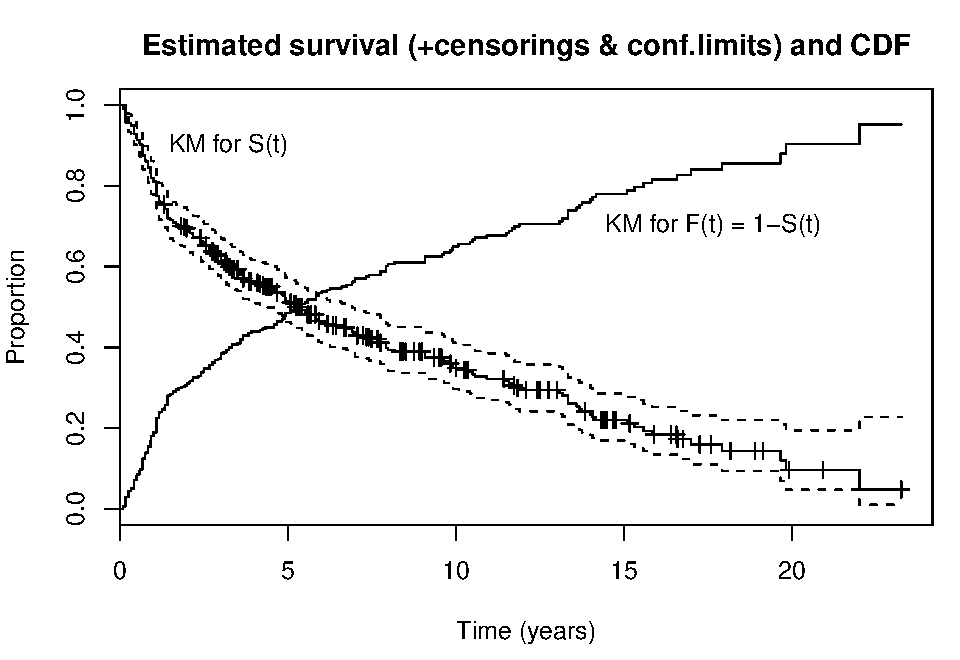
\includegraphics[width=1.0\textwidth]{orcaKM1} 
\end{figure}

\end{frame}


\begin{frame}
   \frametitle{Competing risks model: causes of death}
   
\begin{itemize}
\item
Often the interest is focused on the risk or hazard of dying 
from one specific cause.
\medskip
\item
That cause may eventually not be realized, because
a \textbf{competing cause} of death hits first.

\bigskip

\begin{center}
\setlength{\unitlength}{0.65pt}
\begin{picture}(400,190)
  \thicklines
  \put(  0, 115){\makebox(120,50)[b]{\footnotesize{(lex.Cst = 0)}}}
  \put(  0, 80){\framebox(130,60){Alive}}
  \put(  0, 80){\makebox(120,50)[b]{\footnotesize{(lex.Xst = 0)}}}
  %
  \put(230,130){\framebox(180,50){Dead from cancer}}
  \put(230, 130){\makebox(120,40)[b]{\scriptsize{(lex.Xst = 1)}}}
  %  \put(170, 97){(Cause-specific hazards)}
  \put(230, 30){\framebox(180,50){Dead, other causes}}
  \put(135,125){\vector(3, 1){90}}
  \put(230, 30){\makebox(120,30)[b]{\scriptsize{(lex.Xst = 2)}}}
%  \put(295,155){\vector(0,-1){100}}
  \put(135, 85){\vector(3,-1){90}}
  \put(165,157){\makebox(0,0)[b]{$\lambda_1(t)$}}
  \put(165, 53){\makebox(0,0)[t]{$\lambda_2(t)$}}
% \put(285,105){\makebox(0,0)[t]{$\nu$}}
\end{picture}
\end{center}
\item
 Generalizes to several competing causes.
 \end{itemize}
% Illness-death model. Little boxes with arrows.\\
% (The mortality of lung cancer patients ($\nu$) not relevant here).
\end{frame}

\begin{frame}
\frametitle{Competing events \& competing risks}

In many epidemiological and clinical contexts there are
competing events that may 
occur before the target event and remove the person from 
 the population at risk for the event, \textit{e.g.}

\begin{itemize}
\item \textit{target event}: occurrence of endometrial cancer,
 \textit{competing events}: hysterectomy or death.
\medskip
\item \textit{target event}: relapse of a disease \\
(ending the state of remission), \\
 \textit{competing event}: death while still in remission.
 
% \medskip
\item \textit{target event}: divorce, \\ 
 \textit{competing event}: death of either spouse.
 
\end{itemize}

\end{frame}

\begin{frame}[fragile]
\frametitle{Event-specific quantities}

\textbf{Cumulative incidence function} (CIF) or \\
 %\textbf{subdistribution function} for event $c$:
\[  F_c(t) = P(T \leq t \text{ and } C = c ), \quad c = 1,2,  \]
%{subdensity function} $f_c(t) = dF_c(t)/dt$ 

\medskip
From these one can recover
\begin{itemize}
\item
$F(t) = \sum_{c} F_c(t)$, CDF of event-free survival time $T$, \textit{i.e.} 
cumulative risk of any event by $t$.
\medskip
\item
$S(t) = 1 - F(t)$, \textbf{event-free survival function}, \textit{i.e.} probability of avoiding all events by $t$, but $S(t) \ne F_1(t)+F_2(t)$
\end{itemize}
\end{frame}


\begin{frame}[fragile]
\frametitle{Event-specific quantities (cont'd)}

\textbf{Event-} or \textbf{cause-specific hazard function}
\begin{align*}
 \lambda_c(t) & =  \underset{\Delta\to 0}{\lim} 
    \frac{P(t < T \le t+\Delta \text{ and } C = c \mid T > t)}{\Delta}  \\
        & =  \frac{f_c(t)}{1-F(t)}
\end{align*}
% \underset{\Delta\to 0}{\lim} \frac{F_c(t+\Delta) - F_c(t)}{S(t)}/\Delta

CIF   =  risk of event $c$ over risk period $[0,t]$ in the presence of competing risks, also obtained 
$$ F_c(t) = \int_0^t \lambda_c(v) S(v) dv, \quad c = 1,2, $$
\end{frame}

\begin{frame}
\frametitle{Warning of ``net risk'' and ``cause-specific survival''}

\begin{itemize}                              
\item
The ``\textbf{\textit{net risk}}'' of outcome $c$ by time $t$, 
assuming hypothetical elimination of competing risks,
is often defined as
\begin{center}
$ F_1^*(t) = 1 - S_1^*(t) = 1- \exp\{ - \Lambda_1(t) \} \ne S(t) $
% =1 - \exp\left\{ - \int_0^t h_c(v) dv \right\},  $$
\end{center}
\medskip
\item
In clinical survival studies, function 
$S_1^*(t)$ is often called ``\textbf{\textit{cause-specific survival}}'',
%and estimated by KM, but treating competing deaths
%as censorings.
or ``\textbf{\textit{net survival}}''
\medskip
\item
Yet, these *-functions, $ F_1^*(t)$ and $S_1^*(t)$, lack proper probability interpretation when
 competing risks exist.
\medskip
\item
Hence, their use 
%and naive KM estimation 
should be viewed critically
(Andersen \& Keiding, \textit{Stat Med}, 2012)
\end{itemize}
\end{frame}

\begin{frame}
   \frametitle{Example: Risk of lung cancer by age $a$?}
% \vspace*{-1em}
% \[
% \ptxt{Lung cancer before age 75} \ne 1-\e^{-\Lambda(75)}
% \]
% does not take the possibility of death prior to lung cancer into
% account.

\begin{itemize}
% \item 
%  Empirical \textbf{cumulative rate} 
% CR$(a) = \sum_{k < a} I_k \Delta_k$, i.e.
%  ageband-width ($\Delta_k$) weighted 
%  sum of empirical 
%  age-specific incidence rates $I_k$
%  up to a given age $a$ \\
%  = estimate of cumulative hazard $\Lambda_c(a)$.
%  \medskip
 \item 
 Nordcan \& Globocan give 
``\textbf{\textit{cumulative risk}}'' by 75 y of age, computed from 
$1 - \exp\{-\text{CR}(75)\}$, as an estimate  of the probability of 
getting cancer before age $75$ y, 
assuming that death were avoided by that age. This is based on 
deriving ``net risk'' from cumulative hazard:
\begin{center} 
$ F_1^*(a) = 1 - \exp\{ - \Lambda_c(a) \}. $
\end{center}
\medskip
\item
Yet, cancer occurs in a mortal population.
\medskip
\item
As such CR$({75})$ is a sound age-standardized summary 
 measure for comparing cancer incidence across populations 
 based on a neutral standard population.
\end{itemize}

\end{frame}

\begin{frame}
\frametitle{Example. Male lung cancer in Denmark}

Event-specific hazards: $\lambda_1(a)$ (lung cancer) death $\lambda_2(a)$ by age estimated by age-spec. rates.

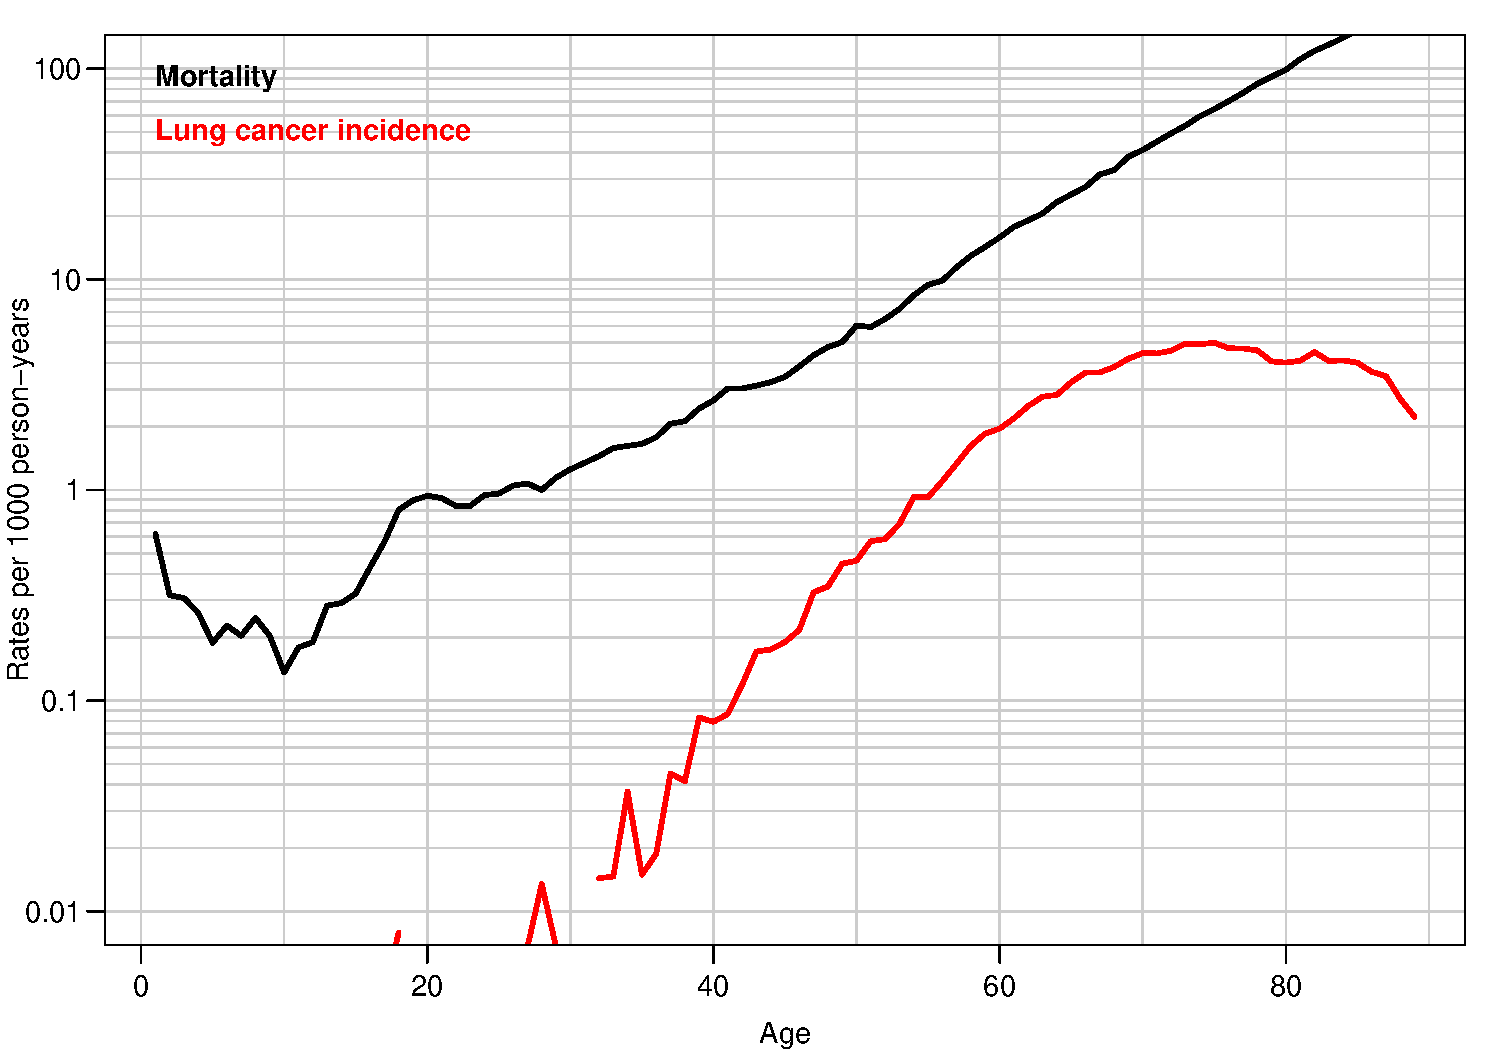
\includegraphics[height=6.5cm]{lung-ca-rates}
\end{frame}

\begin{frame}
\frametitle{Cumulative incidence of lung cancer by age}

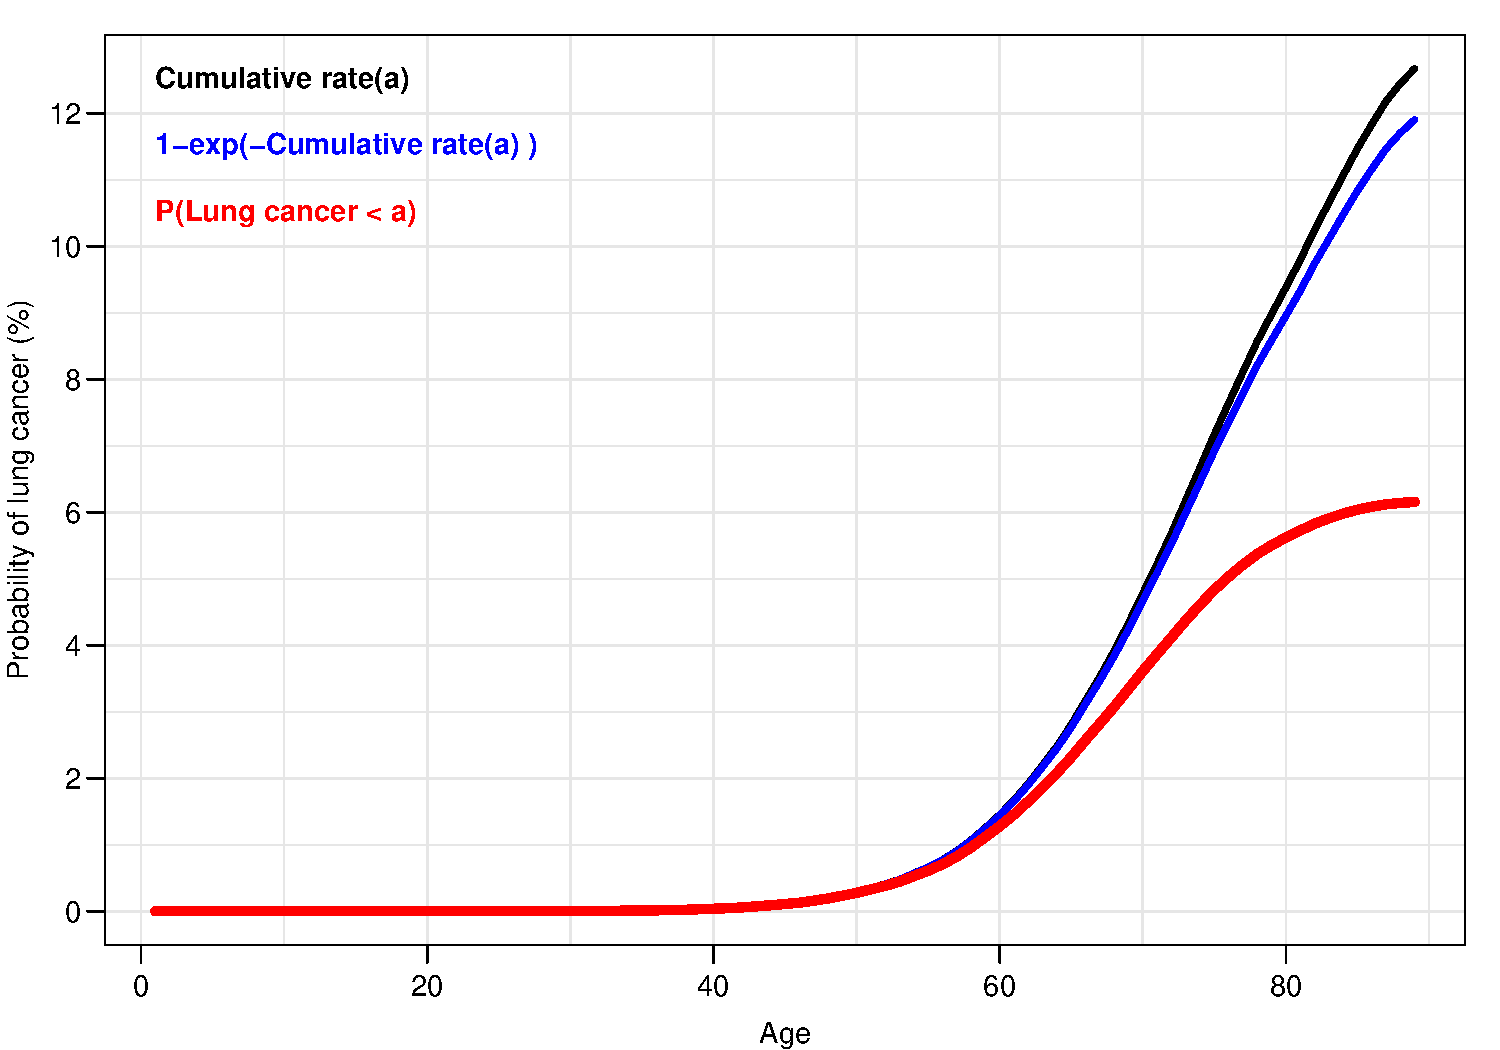
\includegraphics[height=6.5cm]{lung-ca-prob}

Both \text{CR} and $1 - \exp(- \text{CR})$ tend to \\
 overestimate the real cumulative incidence CI after 60 y.
\end{frame}


\begin{frame}[fragile]
\frametitle{Analysis with competing events}

Let $U_i$ = censoring time, 
% $\quad B_i$ = time of entry to follow-up (often $B_i = 0$),  \\
$T_i$ = time to first event, and \\
$C_i$ = variable for event 1 or 2. %, $i=1, \dots, n$. \\
We observe 
\begin{itemize}
\item $y_i = \text{min}\{ T_i, U_i \}$, \textit{i.e.}
the exit time, and
\item
 $ \delta_{ic} = 1_{ \{ T_i < U_i \ \& \ C_i = c\} }$, 
  indicator (1/0) for \\ 
  event $c$ being first observed, $c=1,2$. 
\end{itemize}


Non-parametric estimation % $\widetilde{F}_c(t)$ 
of CIF

\begin{itemize}
\item
Let $t_1 < t_2 < \dots < t_K$ be the $K$ distinct 
time points at which any outcome event was observed, \\ Let also
 $\widetilde{S}(t)$ be KM estimator for overall $S(t)$. 
\medskip
\item
\textbf{Aalen-Johansen estimator} (AJ) for the cumulative incidence function $F(t)$
should be used 
%is obtained as$$ \widetilde{F}_c(t) 
%   = \sum_{t_k \leq t} \frac{D_{kc}}{n_k} \times \widetilde{S}(t_{k-1}),
%   \quad\text{where}
%$$
%$n_k$ = size of the risk set at $t_k$ $(k=1, \dots, K)$,
%\\
%$D_{kc}$ = no. of cases of event $c$ observed  at $t_k$.
%\medskip
%\item
% \medskip
%Naive KM estimator $\widetilde{F}^*_c(t)$ of ``net survival'' treats  
%competing events occuring first as censorings:  
%$$  \widetilde{F}^*_c(t) = 1 - \widetilde{S}^*_c(t)
%  = 1 - \prod_{t_k \leq t} \frac{n_k - D_{kc}}{n_k} $$
\end{itemize}

\end{frame}

\begin{frame}[fragile]

\frametitle{R tools for competing risks analysis}

Package \texttt{mstate}
\begin{itemize}
% \item Covers even more general multi-state set-ups.
%  \pause
%  \medskip
\item \texttt{Cuminc(time, status, ...)}:  \\
 AJ-estimates (and SEs) for each event type 
 % from observed follow-up times and events
  (\texttt{status}, value 0 indicating censoring)
\end{itemize}
Package \texttt{cmprsk}
\begin{itemize}
\item \texttt{cuminc(ftime, fstatus, ...)} 
  computes CIF-estimates,  % in \texttt{mstate},
   \texttt{plot.cuminc()} plots them. 
  \medskip
\item \texttt{crr()}
 fits Fine--Gray models for 
the hazard $\gamma_c(t)$ of the subdistribution
\end{itemize}   
Package \texttt{Epi} -- \texttt{Lexis} tools for multistate analyses
\begin{itemize}
\item  will be advertised by Bendix!
\end{itemize}

\end{frame}

\begin{frame}[fragile]
\frametitle{Ex. Survival from oral cancer}

\begin{itemize}
\item
Creating a {\tt Lexis} object with two outcome events and \\ 
obtaining a summary of transitions
\end{itemize}
\small
\begin{verbatim}
> orca.lex <- Lexis(exit = list(stime = time), 
           exit.status = factor(event, 
    labels = c("Alive", "Oral ca. death", "Other death") ),
                  data = orca)

> summary(orca.lex)  
Transitions:
     To
From    Alive Oral ca. Other  Records:  Events: Risk time:  Persons:
  Alive   109      122   107       338      229    1913.67       338
\end{verbatim}
\normalsize

\end{frame}

\begin{frame}[fragile]
\frametitle{Box diagram for transitions}

Interactive use of function {\tt boxes()}.
\small
\begin{verbatim}
> boxes(orca.lex)
\end{verbatim}
\begin{center}
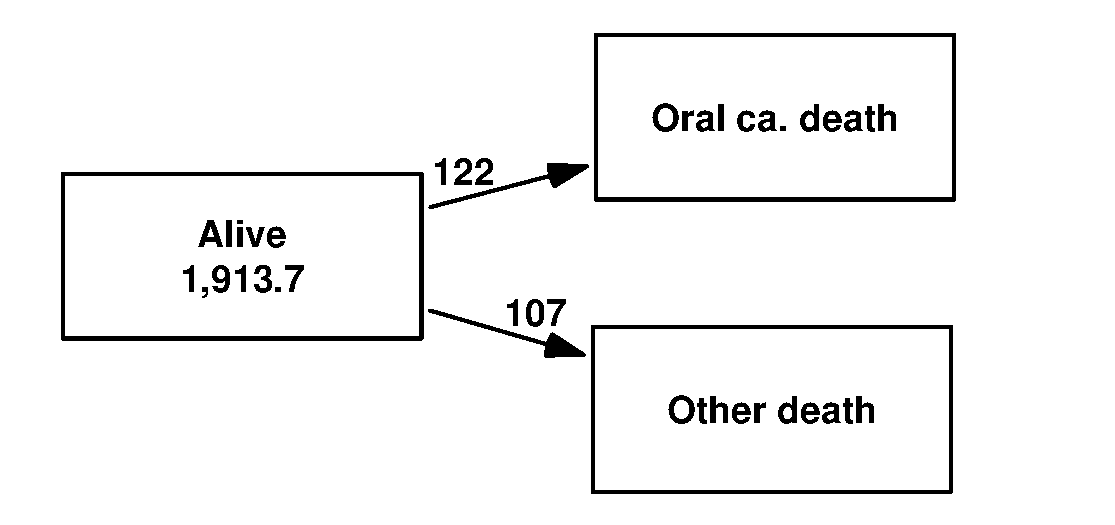
\includegraphics[height=6cm]{orca-boxes}
\end{center}
\normalsize

\end{frame}

\begin{frame}[fragile]
\frametitle{Ex. Survival from oral cancer}
\begin{itemize}
\item
AJ-estimates of CIFs (solid) for both causes.
\item
Naive KM-estimates of CIF (dashed) $>$ AJ-estimates 
\item
CIF curves may also be stacked (right).  
\end{itemize}
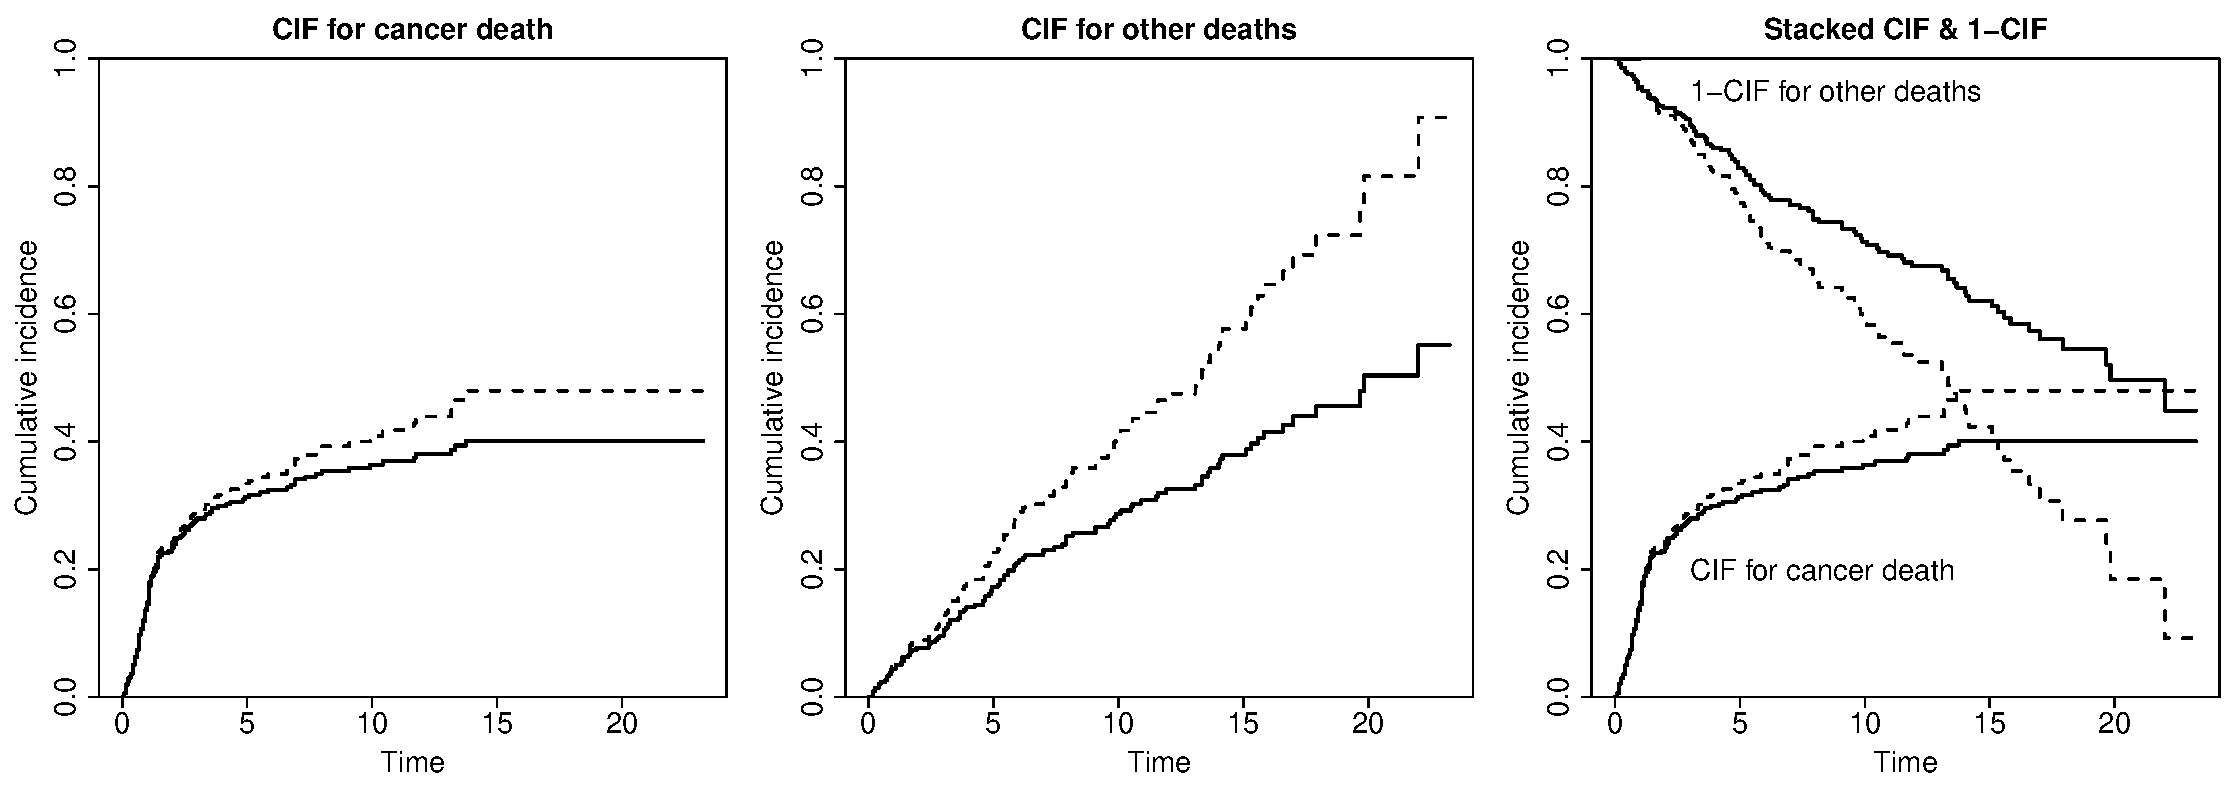
\includegraphics[width=\textwidth]{orcaCI1}

\textbf{NB.} The sum of the naive KM-estimates of CIF exceeds 100\% at 13 years! 
\end{frame}

\begin{frame}[fragile]
\frametitle{Ex. CIFs by cause in men and women}

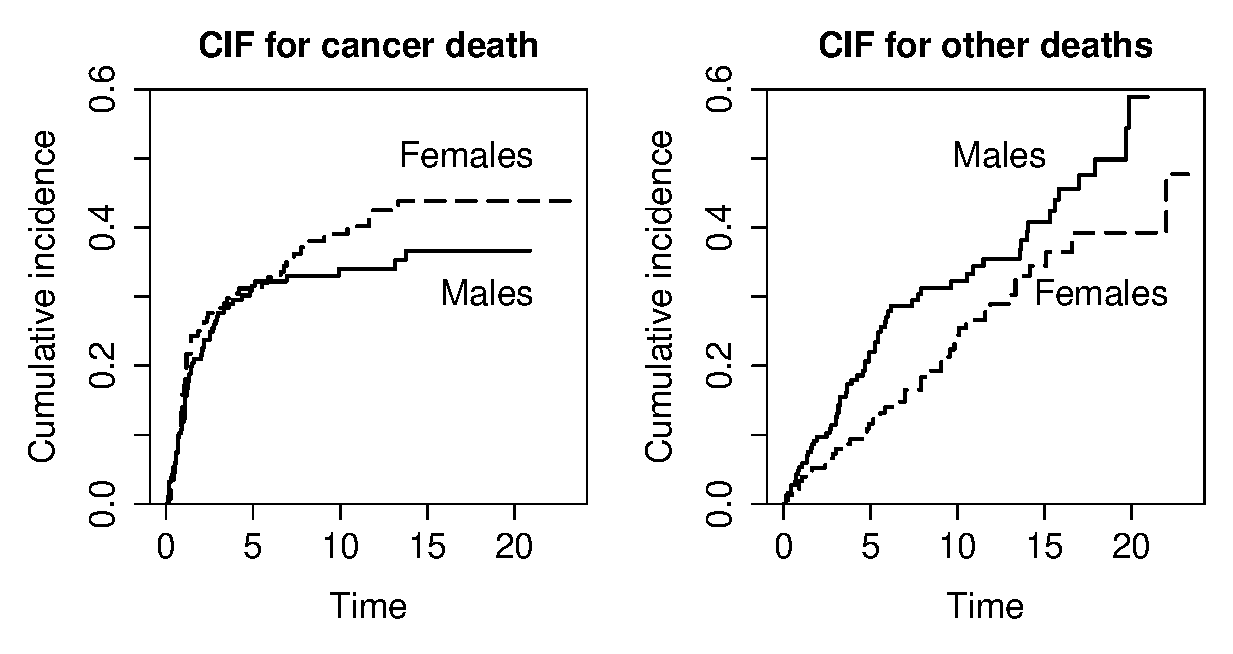
\includegraphics[width=\textwidth]{orcaCI2}

CIF for cancer higher in women (chance?) but for other causes
higher in men (no surprise).

\end{frame}

\begin{frame}

\frametitle{Regression models for time-to-event data}


Regression models for hazards can be defined \textit{e.g.} for 
\begin{itemize}
% \item[(a)] survival times directly 
% $$ \log(T_i) = \eta_i + \epsilon_i, \quad\text{s.t. } 
% \epsilon_i \sim F_0(t; \alpha)$$ 
% where $F_0(t; \alpha)$ is some baseline model, 
% \medskip
% \pause
\item[(a)] hazards, multiplicatively: $$ 
\lambda_i(t) = \lambda_0(t; \alpha) r(\eta_i), \quad\text{where}$$
$\lambda_0(t; \alpha)$ = baseline hazard and \\
$r(\eta_i)$ = relative rate function, typically $\exp(\eta_i)$
\medskip
\pause
\item[(b)] hazards, additively: 
$$ \lambda_i(t) = \lambda_0(t; \alpha) + \eta_i. $$
\end{itemize}
\end{frame}


\begin{frame}
\frametitle{Relative hazards model or Cox model}

In model (b), the baseline hazard $\lambda_0(t,\alpha)$ may be given a parametric form (\textit{e.g.} Weibull) or
a piecewise constant rate (exponential) structure.

\bigskip
Often a parameter-free form $\lambda_0(t)$ is assumed. Then
\[
  \lambda_i(t) = \lambda_0(t) \exp(\eta_1),
\]
specifies the \textbf{Cox model} or the \textbf{semiparametric proportional hazards model}.

\bigskip
$\eta_i = \beta_1 x_{i1} + \dots + \beta_p x_{ip}$ not depending on time.  

\bigskip
Generalizations: \textbf{time-dependent} \\ covariates $x_{ij}(t)$

% For exponential model, $\lambda_0(t) = \lambda_0$.

% Piecewise exponential model $\to$ constant baseline
% hazard in successive intervals:   
% \[ 
% \lambda_0(t) = \lambda_{0k}, \mbox{ for } 
% a_{k-1}} < t \leq a_k, \quad k = 1, 2, \dots, K 
% \]

\end{frame}


\begin{frame}
\frametitle{PH model: interpretation of parameters}

Present the model explicitly in terms of $x$'s and $\beta$'s.
\[
\lambda_i(t) = \lambda_0(t)  \exp({\beta_1 x_{i1} + \dots +
\beta_p x_{ip}})
\]
Consider two individuals, $i$ and $i'$, having the same values of all
other covariates except the $j^{\text{th}}$ one.

\bigskip
The ratio of hazards is constant:
$$  \frac{\lambda_i(t)}{\lambda_{i'}(t)} = \frac{\exp( \eta_{i}) }{\exp(\eta_{i'})}
= \exp \{ \beta_j(x_{ij}-x_{i'j}) \} . $$
Thus $e^{\beta_j} = \text{HR}_j$ = \textbf{hazard ratio} or relative rate
 associated with
 a unit change in covariate $X_j$.

\end{frame}

\begin{frame}[fragile]
\frametitle{Ex. Total mortality of oral ca. patients}

Fitting Cox models with sex and sex + age.
\small
\begin{verbatim}
> cm0 <- coxph( suob ~ sex, data = orca)
> summary( cm0)
        coef exp(coef) se(coef)    z Pr(>|z|)
sexMale 0.126     1.134    0.134 0.94     0.35
        exp(coef) exp(-coef) lower .95 upper .95
sexMale      1.13      0.882     0.872      1.47

> cm1 <- coxph( suob ~ sex + age, data = orca)
> summary(cm1)
        exp(coef) exp(-coef) lower .95 upper .95
sexMale      1.49      0.669      1.14      1.96
age          1.04      0.960      1.03      1.05
\end{verbatim}
\normalsize
The M/F contrast visible only after age-adjustment.
\end{frame}

\begin{frame}[fragile]
\frametitle{Predictions from the Cox model}
\begin{itemize}
\item
Individual survival \textit{times} cannot be predicted
but ind'l survival \emph{curves} can.
PH model implies:
\[
S_i(t) = [S_0(t) ]^{\exp(\beta_1 x_{i1} +\ldots+\beta_p x_{ip})}
\]
\item
Having  estimated $\beta$ by partial likelihood, 
the baseline $S_0(t)$ is estimated by Breslow method 
\item 
\medskip
 From these, a survival curve for an individual
with given covariate values is predicted.
\item
\medskip
In R: 
\texttt{pred <- survfit(mod, newdata=...)} 
and \texttt{plot(pred)}, where \texttt{mod} is the fitted
\texttt{coxph} object, 
and \texttt{newdata}  
specifies the covariate values.
\end{itemize}
\end{frame}

\begin{frame}
\frametitle{Modelling with competing risks}

% When more than one outcome are operating,
% one may consider the 
Main options, providing answers to different questions.

\begin{itemize}
\item[(a)]
  Cox model for event-specific hazards $\lambda_c(t) = f_c(t)/[1-F(t)]$, when \textit{e.g.} the interest is in the biological effect of the prognostic factors on the fatality of the very disease that often leads to the relevant outcome.  
  \bigskip 
\item[(b)]
 \textbf{Fine--Gray model} for the hazard  of the subdistribution $\gamma_c(t) = f_c(t)/[1-F_c(t)]$ 
  when we want to assess the impact of the factors on the overall cumulative incidence of event $c$.  \\
  -- Function \texttt{crr()} in package \texttt{cmprsk}. 
\end{itemize}

\end{frame}


\end{document}
